%
% File eacl2017.tex
%
%% Based on the style files for ACL-2016
%% Based on the style files for ACL-2015, with some improvements
%%  taken from the NAACL-2016 style
%% Based on the style files for ACL-2014, which were, in turn,
%% Based on the style files for ACL-2013, which were, in turn,
%% Based on the style files for ACL-2012, which were, in turn,
%% based on the style files for ACL-2011, which were, in turn, 
%% based on the style files for ACL-2010, which were, in turn, 
%% based on the style files for ACL-IJCNLP-2009, which were, in turn,
%% based on the style files for EACL-2009 and IJCNLP-2008...

%% Based on the style files for EACL 2006 by 
%%e.agirre@ehu.es or Sergi.Balari@uab.es
%% and that of ACL 08 by Joakim Nivre and Noah Smith

\documentclass[11pt]{article}
\usepackage{eacl2017}
\usepackage{times}
\usepackage{url}
\usepackage{latexsym}
\usepackage{natbib}
\usepackage{amsmath}
\usepackage{subfigure}
\usepackage{graphicx}

\eaclfinalcopy % Uncomment this line for the final submission
%\def\eaclpaperid{***} %  Enter the acl Paper ID here

%\setlength\titlebox{5cm}
% You can expand the titlebox if you need extra space
% to show all the authors. Please do not make the titlebox
% smaller than 5cm (the original size); we will check this
% in the camera-ready version and ask you to change it back.

\newcommand\BibTeX{B{\sc ib}\TeX}

\title{Learning to Negate Adjectives with Bilinear Models}
% Learning to Negate Adjectives with Relational Antonym Encoders
% Learning to Negate Adjectives with Continuous Class-Conditional Relational Encoders

\author{First Author \\
  Affiliation / Address line 1 \\
  Affiliation / Address line 2 \\
  Affiliation / Address line 3 \\
  {\tt email@domain} \\\And
  Second Author \\
  Affiliation / Address line 1 \\
  Affiliation / Address line 2 \\
  Affiliation / Address line 3 \\
  {\tt email@domain} \\}

\date{}

\begin{document}
\maketitle
\begin{abstract}
 TODO
\vspace{15mm}
\end{abstract}

\section{Introduction}

Identifying antonyms in a vector space model is a notoriously
challenging task, because the vectors for related words of opposite
polarity, such as {\it hot} and {\it cold}, are close to each other in
most commonly-used word embedding models. Retrofitting embeddings to
enhance lexical contrast, or learning embeddings with lexical contrast
as a secondary objective \citep{pham:15,nguyen:16,mrksic:16}, has been
shown to improve the overall embedding quality as well as the ability
to distinguish synonyms from antonyms. In this paper we adress a
different task: given an arbitrary set of word embeddings, we wish to
learn a negation function which returns an antonym for a given
word. This task is relevant for composing larger units of meaning,
where a phrase such as {\it not cold} might need to be assigned a
vector space representation.

We focus on negating adjectives, and treat negation as prediction of a
one-best antonym. For example, given the expression {\it not
  talkative} and the vector $\overrightarrow{\textit{talkative}}$, the negation
function should return a word from the set {\it quiet, taciturn,
  uncommunicative}, etc.

% More nuanced treatmeants of antonym negation are possible; e.g. the meaning of {\it not
%   hot} can include {\it cool,
%   tepid, warm} etc. depending on the context \citep{hermann:13}.
% [TODO  Baroni] [TODO maybe a linguistic cite]

% Previous work on antonymy has suggested that, while antonyms are
% distributionally similar, there are differences which can be
% exploited. 
Semantically, antonyms share a domain---e.g. {\it
  temperature}, but differ in their value---e.g. {\it cold}
\citep{turney:12,hermann:13}. The challenge for negation is to learn
which features need to change, and in what direction, to change the
value while retaining the semantic domain of the
word. \citet{santus:15} propose that antonyms differ along their less
salient shared contexts, using an LMI-based measure for distinguishing
antonymy from other binary relations; crucially, however, relation
classification on word pairs does not predict an antonym given a word.

In this paper we exploit the semantic neighbourhood of each adjective
as a stand-in for the domain. We hypothesize that the relevant
features for negating, say, a temperature adjective, differ from those
for an emotion adjective. Therefore, we learn a function that uses a
vector representing the neutral semantic context of the input
word. Moreover, a negation function must be (informally) involuntory,
i.e. its own inverse, so it must detect the ``direction'' in which the
input word is more extreme than the neutral vector. This approach is inspired by \citet{kruszewski:16},
 who observe that nearest neighbours in a vector space are a good approximation for the 
alternatives that humans produce for negation.

By using a bilinear relational neural network architecture used to
identify transformations in computer vision, we are able to learn a
negation relevant function. Our model outperforms other variants on a
GRE multiple choice taks, and more importantly learns to produce a
one-best antonym with high precision.


\section{Relational Encoders}

\begin{figure*}[h!t]
\subfigure{
 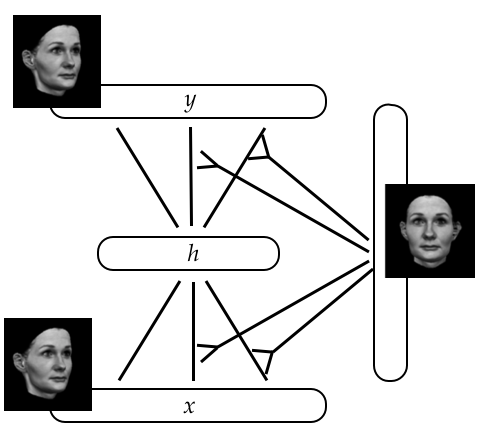
\includegraphics[width=0.3\textwidth]{rae}
}
\label{f:arch}
\caption{Neural network architectures for RAE, CCRAE, CCCRE.}
\end{figure*}



\subsection{Relational Autoencoders: Background}

Relational autoencoders (RAE), also known as gated autoencoders (GAE),
have been used in computer vision to learn representations of
transformations between images, such as rotation or translation \citep{memisevic:07,memisevic:12,memisevic:13}. RAEs
are a type of {\it gated network}, in which multiplicative connections
between two related inputs are used for prediction or representation
learning. The ``gating'' of one image vector by another allows the feature detectors to concentrate on the correspondences between the related images, rather than being distracted by the differences between untransformed images (Figure~\ref{f:arch}). The key is bilinear connections; there is a weight for every pair of units in the input vector and gate vector. For an overview of RAEs see \citet{memisevic:13,sigaud:15}.
% The connections are known as bilinear because for an image x and its rotated image y, f(y) is a linear function of x, and vice versa.
% The connections are symmetric, but one input is usually considered primary and the other the gate.

We note that despite the terminology, the gates in an RAE perform a somewhat different function than in an LSTM \citep{lstm}. Both network architectures use a nonlinearity to modulate the contents of a product; in an RAE this is an outer (bilinear) product while in an LSTM it is a Hadamard (element-wise) product. However, LSTM gates are memory gates which represent an internal hidden state of the network, while RAE gates are part of the input to the network.

An AE can be defined as follows (we omit bias terms for the sake of simplicity), where $\mathrm{W_e}$ are the encoder weights and $\mathrm{W_d}$ as the decoder weights. In autoencoders it is typical for them to be tied so that $\mathrm{W_d} = \mathrm{W_e}^T$.

\begin{equation}
\begin{split}
h & = f(x) = \sigma (\mathrm{W_e}x ) \\
y & = g(h) = \mathrm{W_d}h
\end{split}
\end{equation}

For an RAE, we have two inputs $x$ and $z$. Instead of a weight matrix $W$ we have a weight tensor $\overline{\mathrm{W}} \in R^{n_H \times n_X \times n_Z}$.  The RAE is defined as follows.

\begin{equation}
\begin{split}
h & = f(x, z) = \sigma ((\overline{\mathrm{W_e}}z)x) \\
y & = g(h, z) = \sigma ((\overline{\mathrm{W_d}}h)z)
\end{split}
\end{equation}

\citet{rudy:15} introduce a class-conditional gated autoencoder in which the gate is a one-hot class label, rather than a transformed version of the input image. For example, in the MNIST task the label represents the digit. This is like training an autoencoder per class but with weight sharing across classes. See Figure~\ref{f:arch}(b).

\subsection{Continuous Class-Conditional Relational Encoders}

Our bilinear model is a continuous class-conditional relational encoder (CCCRE). The model architecture is the same as an RAE with untied encoder and decoder weights. However, the training signal differs from a classic RAE in two ways. First, it is not an autoencoder, but simply an encoder, because it is not trained to reproduce the input but rather to transform the input to its antonym. Second, the encoder is class-conditional in the sense of \cite{rudy:15}. In a classic RAE the input and gate are related according to a transformation, but in a class-conditional AE the gate represents the class. Unlike the one-hot gates of \cite{rudy:15}, our gates, representing the semantic domain of the input vector, are real-valued. See Figure~\ref{f:arch}(c).

\section{Experiments}

\subsection{Models}


We compare the CCCRE with (1) an Untied Encoder with a bottleneck. (1) a simple feed-forward network that uses no neutral context gate. (2) a feed-forward network where the input consists of the word vector concatenated with the gate vector. The network therefore has information about the semantic network and can relate the word and the gate by way of the connections to the hidden layer,  but has no bilinear connections. (3) auto-encoders with and without the concatenated gate as input. We did not find denoising to help in any of our models and do not use it.

Baselines are: cosine similarity, linear map.

\section{Experimental Settings}


We use the publicly-available\footnote{\url{https://code.google.com/archive/p/word2vec/}} embeddings obtained using the skip-gram with negative sampling model of Mikolov et al. (2013). These are 300-dimensional and were trained on part of the Google News dataset.

Antonym training data was obtained from WordNet. We started with all adjectives having antonyms in WN. We expanded the list by taking WN synonyms of the antonyms in these pairs. This resulted in an order of magnitude more training data, approximately 20K pairs (depending on setting), without introducing too much noise into the training data. Any input word in the test set (see below) was excluded from the INPUT side of the training data. We did not exclude it as a target in the training data. We also did not exclude cohyponyms of the test input words, since the theory is that the network needs these examples to learn the gates / contexts. That is, if 'cold' is in the test set, the model learns how to negate it by learning how to negate other temperature words.

Neutral context gates were obtained under three conditions. First, we took all WordNet cohyponyms of the adjective\footnote{includes adjective satellite} sense of input word $w$, where cohyponyms include: other lemmas in the synset, children of attribute, synonyms, antonyms, synonyms of the antonyms, similar-tos. If there were fewer than 10 cohyponyms in WordNet, we increased the number to 10 with non-overlapping nearest neighbours from the original vector space. The gate is the centroid of these vectors.

The second condition is {\bf unsupervised} gates. Here we do not use WN to find the semantic neighbourhood. We use the ten nearest neighbours from the original vector space. However, the target antonym is still supervised.

In the third condition, which we call {\bf restricted}, we remove all cohyponys of test input words from the training data. This is to test how important it is to have training examples with similar gates. For example, if {\it cold} is a test word, we remove {\it hot, cold, tepid, cool} etc. from the training data.

We used MSE loss. Hyperparameters were tuned on the GRE development set. The feed forward and CCCRE networks have hidden layers of 600 units, while the UAE has a hidden layer of 150, and 300 for UAE-Concat. Minibatch size was 48 for bilinear networks and 16 for the others. Number of epochs 400 for feed-forward, 200 for bilinear, 300 for UAE, 100 for linear. Optimization adadelta with $\rho = 0.95$.


\begin{table}[t!]
% \centering
% \small
\begin{tabular}{lccc}
\hline
 & \multicolumn{3}{c}{\bf Training Condition} \\
\bf Method & \bf Stand. & \bf Unsup. & \bf Restr. \\
\hline
\hline
Random & 0.20 & --- & --- \\
Cosine & 0.50 & --- & --- \\
Linear & 0.56 & & \\
Linear-Concat & 0.66 & & \\
\hline
UE & 0.57 & & \\
UE-Concat & 0.63 & & \\
FF & 0.58 & 0.54 & 0.51 \\
FF-Concat & 0.65 & 0.56 & 0.63 \\
CCCRE & \bf 0.69 & \bf 0.60 & \bf 0.65 \\
\end{tabular} 
\label{t:gre}
\caption{Accuracy on the 367 multiple-choice adjective questions in the GRE test set.}
\end{table}


\section{Evaluation}



\begin{table*}[t!]
\centering
\setlength\tabcolsep{1.5pt}
\begin{tabular}{l|cc|cc|cc|cc|cc|cc|cc|cc|cc|}
\hline
& \multicolumn{6}{c|}{\bf GRE} & \multicolumn{6}{c}{\bf Lenci} \\
& \multicolumn{2}{c|}{\bf Stand.} & \multicolumn{2}{c|}{\bf Unsup.} & \multicolumn{2}{c|}{\bf Restr.} & \multicolumn{2}{c|}{\bf Stand.} & \multicolumn{2}{c|}{\bf Unsup.} & \multicolumn{2}{c}{\bf Restr.} \\
\bf Method & \bf P@1 & \bf P@5  & \bf P@1 & \bf P@5  & \bf P@1 & \bf P@5  & \bf P@1 & \bf P@5  & \bf P@1 & \bf P@5  & \bf P@1 & \bf P@5  \\
\hline
\hline
Cosine & 0.05 & 0.07 & --- & --- & --- & --- & 0.13 & 0.10 & --- & --- & --- & --- \\
Linear & 0.39 & 0.33 & & & & & & & & & & \\
\hline
FF & 0.37 & 0.32 & 0.34 & 0.30 & 0.08 & 0.15 & 0.30 & 0.24 & & & & \\
FF-Concat & 0.36 & 0.30 & 0.46 & 0.40 & 0.37 & 0.34 & 0.34 &  0.26 & & & \\
UE & 0.38 & 0.33 & & & & & 0.28  & 0.22 & & & & \\
UE-Concat & 0.38 & 0.33 & & & & & 0.33 & 0.28 & & & & & \\
CCCRE  & \bf 0.66 & \bf 0.49 & \bf 0.52 & \bf 0.42 & \bf 0.52 & \bf 0.38 & \bf 0.39 & \bf 0.32 & & & & \\
\end{tabular} 
\label{t:prec}
\caption{Precision at ranks 1 and 5 on the GRE and Lenci datasets.}
\end{table*}




We evaluted our models with two experiments. Experiment 1 uses the Graduate Record Examination (GRE) questions of \citet{mohammad:13}. The task is, given an input word, to pick the best antonym out of five options. An example from the development set is shown in (\ref{eqn:gre-ex}), where the input word is {\it piquant} and the correct answer is {\it bland}. We restrict the questions to those in which both input and target words are adjectives.

\begin{equation}
\begin{split}
\textrm{piquant:\ \ } & \textrm{(a) shocking (b) jovial (c) rigorous} \\
& \textrm{(d) merry (e) {\bf bland}}
\label{eqn:gre-ex}
\end{split}
\end{equation}

We evaluate by predicting the antonym for the input word. We measure cosine distance from the predicted vector to each of the five terms in the multiple choice question, and predict the closest term. The results are shown as accuracy, i.e. percentage of questions answered correctly.

Experiment 2 evaluates the precision of the models. Remember that the task is to negate an adjective given its word vector. The most natural criterion for success is whether the model returns a good antonym at rank one, or a number of good antonyms at lower ranks. Following \citep{gorman:05}, we expand our gold standard for evaluation beyond WN, because we found that WN did not have enough coverage. We obtained additional gold standard antonyms from the online version of Roget's 21st Century Thesaurus, Third Edition.\footnote{\url{http://thesaurus.com}} We report precision at ranks 1 and 5. For this evaluation we use two test datasets: the input words from the GRE test set, and a set of 99 adjectives and their antonyms which is part of a dataset collected by Lenci and Benotto acccording to the guidelines of \citet{walde:13}.




\section{Results and Discussion}



Table~\ref{t:gre} gives the results of Experiment 1. The cosine baseline is already fairly strong at 0.50, suggesting that in general about two out of the five choices are closely related to the input word.

The neutral context gate clearly provides useful information for this task, because every linear and non-linear model is helped by concatenation of the gate vector to the input. None of the models without the gate score much higher than the cosine similarity baseline.

Under all conditions, the CCCRE achieves the highest accuracy. In fact it is the only model that beats a linear baseline, which suggests that the bilinear connections are useful for antonym detection.

% The DAE does fairly poorly, suggesting that DAEs are not the right architecture for this task. Putting the input word through a bottleneck may be enough to extract crucial semantic features for reconstructing the original word, but not enough to negate it, where you need to detect where the input word is more extreme than its neutral context.

In the unsupervised setting, in which the neutral context gates are the average of ten nearest neighbour vectors rather than including supervised cohyponyms from WordNet, there is a notable loss of accuracy. This indicates that the makeup of the gates matters and the neighbours are insufficient. For one thing, the centroid of the neighbours may be too close to the vector itself. Even in this setting, however, CCCRE achieves a respectable 0.60 accuracy.


In the restricted setting, FF performs at baseline, suggesting that it is overfitting when it can use the cohyponyms of the test words to learn antonyms. CCCRE still performs quite well, suggesting that it is able to share weights across the different semantic classes.

Overall, this task does not mirror what the CCCRE was designed to do. Inspection of the output shows a number of cases where it fails to predict the specific antonym chosen in the GRE, but the one-best antonym is still very good. [TODO: example]. This is addressed in Experiment 2.


Table~\ref{t:prec} shows precision at ranks 1 and 5 on the GRE and Lenci datasets. In the standard training condition with supervised gates, CCCRE shows an impressive P@1 of 0.66, i.e. two thirds of the time it is able to produce an antonym of the input word as the nearest neighbour of the prediction. All of the other models score less than 0.4. In the other trainin conditions CCCRE retains the ability to give a one-best antonym about half the time.

The Lenci dataset is more challenging [TODO: say why]. However, CCCRE still achieves the highest precision.

% [TODO: we expect the network will have the hardest time negating adjs that don't have a good gate, i.e. a well-defined semantic neighbourhood. Look for some examples.]

\section{Related Work}

\citet{widdows:03} introduces a binary negation function for vector
spaces, e.g. {\it suit NOT lawsuit}, which is used for word sense
disambiguation in Information Retrieval. \citet{turney:12,hermann:13}
propose a multi-part vector representation that separates domain and
value, but this does not allow negation of a word in an arbitrary
vector space. \citet{pham:15,nguyen:16,mrksic:16} use ontologies such
as WN or domain-specific ontologies to retrofit embeddings, or learn
embeddings with a secondary objective, pushing synonyms closer
together and antonyms further apart. This improves the overall vector
space and makes it more likely that close words will be synonyms, but
does not provide a way to find antonyms in the
space. \citet{santus:14a,santus:14b,santus:15} perform synonym-antonym
discrimination using an unsupervised measure based on the relative
salience of shared contexts. This type of relation classification does
not make it possible to negate an arbitrary word. \citet{mohammad:13} use a supervised
thesaurus-based method augmented with co-occurrence statistics on the
GRE task (including nouns and verbs). 
% [TODO Maybe de Marneffe on adjective scales.]

[TODO: vision citations for a couple of applications of RAEs]

%  Turney (2008) proposed a supervised algorithm for the identification of several semantic relations, including synonyms and opposites. The algorithm relied on a training set of word pairs with class labels to assign the labels also to a testing set of word pairs. All word pairs were represented as vectors encoding the fruencies of co-occurrence in textual patterns extracted from a large corpus of web pages. He used the seuential minimal optimization (SMO) support vector machine (M) with a radial basis function (RBF) kernel (Platt, 1998) implemented in Weka (Waikato Environment for Knowledge Analysis) (Witten and Frank, 1999). In the discrimination between synonyms and opposites, the system achieved an accuracy of 75% against a majority class baseline of 65.4%. Mohammad et al. (2008) proposed a method for determining the degree of semantic contrast (i.e. how much two contrasting words are semantically close)  based on the use of thesauri categories and corpus statistics. For each target word pair, they used the co-occurrence and the distributional hypothesis to establish the degree of opposition. Their algorithm achieved an F-score of 0.7, against a random  baseline of 0.2. Mohammad et al. (2013) used an analogical method based on a given set of contrasting words to identify and classify different kinds of opposites by hypothesizing that for every opposing pair of words, A and B, there is at least another opposing pair, C and D, such that A is similar to C and B is similar to D. For example, for the pair
% . Given the existence of contrast, they calculated its degree relying on the
% co-occurrence
%  hypothesis. Their approach outperformed other state-of-the-art measures

\section{Conclusion}

We have shown that a neutral context vector, representing the set of alternatives, improves antonym prediction in linear and non-linear models, and that the multiplicative connections in a bilinear model are effective at learning to negate adjectives. In the broader context of modelling closed-class function words, it is perhaps not too farfetched to imagine that a specialised network with multiplicative connections might be necessary to model these kinds of words.

Our implementation is a simple one, using a full tensor for the bilinear layer, and takes several hours to train on a GPU. Future work will exploit the many options for reducing the number of parameters to be learned \citep{alain:13} and address negation of nouns and verbs, where negation is more likely to involve a probability distribution over alternatives---e.g. {\it didn't run} might mean {\it walk} or {\it amble}---rather than predicting a single best antonym.

\bibliographystyle{myplainnat}
\bibliography{eacl2017}
% \bibliographystyle{eacl2017}


\end{document}
